% =====================================================================
%  第 4 章 围绕拉格朗日子流形 · §4.1–§4.2（ch04a）
%  页段：PDF 129–150（原书 p.119–140）
% =====================================================================
\chapter{围绕拉格朗日子流形}

\section{拉格朗日子流形}

\takeaway{拉格朗日子流形要求维数减半、$\omega$ 在其上为零。余切丛中闭 1-形式的图像与余法丛是典型例子，Weinstein 邻域定理说明局部上只有这一种模型；生成函数又把局部问题归结为奇点的开析。}

% [原文 p.119]
\begin{definition}{4.1}
  辛流形 $(M,\omega)$ 的子流形 $L$ 称为\textbf{拉格朗日子流形}（Lagrangian submanifold），是指
  \[
    \dim L=\frac12\dim M,\qquad \omega|_L=0
  \]
  成立。$n$ 维流形 $L$ 与浸入 $i:L\to M$ 称为\textbf{拉格朗日浸入}（Lagrangian immersion），是指 $i^*\omega=0$。
\end{definition}

拉格朗日子流形是辛几何的中心概念，出现在各种场合。本章尽量多举例子，以展现其一斑。

设 $N$ 为 $n$ 维流形。余切丛 $T^*N$（$2n$ 维）中 $n$ 维子流形的代表例，是微分 1-形式 $u$ 的图像。记作 $\mathrm{Graph}(u)$。把 $\mathrm{Graph}(u)$ 与 $N$ 通过映射 $p\mapsto(p,u(p))$ 等同。

\begin{lemma}{4.2}
  辛形式 $\omega$ 在 $\mathrm{Graph}(u)$ 上的限制等于 $-\rd u$。
\end{lemma}

\begin{corollary}{4.3}
  $\mathrm{Graph}(u)$ 是拉格朗日子流形的充要条件是：$u$ 为闭微分形式。
\end{corollary}

由推论 4.3，余切丛中的拉格朗日子流形可以看作闭微分 1-形式这一概念的推广。

% [原文 p.120]
或者可以看作多值的微分 1-形式。\footnote{闭微分 1-形式 $u$ 大致可写成 $u=\rd f$，故可看作函数的推广。}

\begin{proof}
  令 $\theta=\sum p_i\rd q_i$ 为引理 2.2 的证明中用过的微分 1-形式，即基本形式。$\theta$ 在 $\mathrm{Graph}(u)$ 上的限制是 $u$（由 $\mathrm{Graph}(u)$ 与 $N$ 的等同方式即知）。另一方面 $-\rd\theta=\omega$。
\end{proof}

再举一例。设 $Y$ 为 $N$ 的子流形。令
\[
  T_Y^*N=\{(p,u)\mid p\in Y,\ u\in T_p^*Y,\ \forall V\in T_pN,\ u(V)=0\},
\]
称 $T_Y^*N$ 为\textbf{余法丛}（conormal bundle）。
% [Tutor Note: 原书 p.120 的式子把 $u$ 写成 $T_p^*Y$ 的元素又要求它对所有 $V\in T_pN$ 取零值，二者不能同时成立。通常的定义是 $u\in T_p^*N$ 且 $u|_{T_pY}=0$。]

\begin{lemma*}{4.4}
  余法丛是拉格朗日子流形。
\end{lemma*}
\begin{proof}
  设 $V\in T_{(x,v)}T_Y^*N$（$v\in T_x^*N$，$x\in Y$）。因 $\pi_*(V)\in T_xN$，故 $\theta(V)=v(\pi_*(V))=0$。因此 $\theta$ 到 $T_Y^*N$ 的拉回为 $0$。又 $\rd\theta=-\omega$，故得引理。
\end{proof}

引理 4.4 局部地给出了所有拉格朗日子流形。表述这一事实的是下一定理。

\begin{theorem*}{4.5}
  （Weinstein [384]）设 $(M,\omega_M)$ 为辛流形，$L$ 为其拉格朗日子流形。此时存在 $T^*L$ 的 $0$ 的邻域 $U$ 与 $L$ 在 $M$ 中的邻域 $V$ 之间的辛同胚 $\Psi:U\to V$，且 $\Psi$ 在 $0$ 截面上的限制是到 $L$ 的恒等映射。
\end{theorem*}
\begin{proof}
  设 $U^+$ 为 $0$ 截面的充分小邻域。$TT^*L$ 到 $L$（$=0$ 截面）的限制与 $TM$ 到 $L$ 的限制，连同辛形式在内是同构的。因此存在微分同胚 $\Psi':U^+\to V\subset M$，它在 $0$ 截面上的限制是到 $L$ 的恒等映射，且 $\Psi'^*\omega_M$ 在 $0$ 截面上与 $U^+\subset T^*L$ 的辛形式 $\omega_{T^*L}$ 一致。令 $\omega_\tau=\tau\Psi'^*\omega_M+(1-\tau)\omega_{T^*L}$。与 Darboux 定理或 Moser 定理的证明同样，可以证明存在 $U\subset U^+$ 与 $\Phi_\tau:U\to U^+$，使 $\Phi_\tau^*\omega_\tau=\omega_{T^*L}$，且 $\Phi_\tau$ 在 $0$ 截面上为恒等映射。令 $\Psi'\circ\Phi_1=\Psi$ 即可。
\end{proof}

% [原文 p.121]
下一条引理对于理解拉格朗日子流形在辛几何中的意义很重要。设 $(M,\omega_M)$、$(N,\omega_N)$ 均为 $2n$ 维辛流形。微分 2-形式 $\pi_1^*\omega_M-\pi_2^*\omega_N$ 在直积 $M\times N$ 上确定辛结构。

\begin{lemma*}{4.6}
  设 $\Phi:M\to N$ 为辛同胚。则 $\mathrm{Graph}(\Phi)=\{(x,\Phi(x))\mid x\in M\}$ 是 $(M\times N,\pi_1^*\omega_M-\pi_2^*\omega_N)$ 的拉格朗日子流形。
\end{lemma*}
\begin{proof}
  由 $p\mapsto(p,\Phi(p))$ 把 $M$ 与 $\mathrm{Graph}(\Phi)$ 等同，则 $\pi_1^*\omega_M-\pi_2^*\omega_N$ 在 $\mathrm{Graph}(\Phi)=M$ 上的限制是 $\omega_M-\Phi^*\omega_N$。$\Phi$ 是辛同胚，故 $\omega_M-\Phi^*\omega_N=0$。
\end{proof}

把复几何与辛几何相比，会注意到与全纯映射相当的概念暂时在辛几何中并不存在。也就是说，两个辛流形之间的映射 $\Phi:M\to N$ 与辛结构“整合”该如何表述并不明确。换言之，试图构造辛流形的范畴时，态射应当是什么并不清楚。另一方面，只有辛同胚这一概念是被定义了的。

看了引理 4.6 就会想到：把“$(M\times N,\pi_1^*\omega_M-\pi_2^*\omega_N)$ 的拉格朗日子流形”视为“$M\to N$ 的辛映射”也许不错（这里 $M$ 的维数与 $N$ 的维数不必一致）。但这样定义的话，“辛映射”并不是集合论意义上的 $M$ 到 $N$ 的映射。把 $(M\times N,\pi_1^*\omega_M-\pi_2^*\omega_N)$ 的拉格朗日子流形称为\textbf{拉格朗日对应}（Lagrangian correspondence）。

拉格朗日对应的想法，在辛几何的量子化接触变换（quantized contact transform）与傅里叶积分算子（Fourier integral operator）的应用中也很重要。

\begin{remark}{4.7}
  把 $M\times N$ 的子流形看作 $M\to N$ 的映射，这一想法在数学的许多地方出现，是重要的想法。代数几何中循环的对应（cycle correspondence）就是一例，它与 motive（动机）的想法有关。
% [Tutor Note: 原书 p.121 起把这一思考方式串到 Fourier–Mukai 变换、Hecke 作用素与中岛启的模空间构造；读时可留意“对应”都是“子流形即多值映射”这一原型的变形。]

% [原文 p.122]
  与镜像对称或弦理论的对偶性关系很深的傅里叶–向井变换（Fourier–Mukai transform，参照 [266] 等），以及数论中的 Hecke 作用素，也是其例。此外，中岛启基于用模空间作对应来构造各种代数结构的工作 [278], [279], [280]，大约也属于与之相关的例子。本书第 5、6 章的结构的主要工具，正是通过模空间的对应。这些例子实际上——包括拉格朗日子流形的例子——被认为都通过某种“对偶性（duality）”相互转换。
\end{remark}

举一个拉格朗日对应的例子。设 $(M,\omega_M)$ 为辛流形，假设紧李群 $G$ 在 $M$ 上有哈密顿作用。$f:M\to\mathfrak{g}^*$ 为动量映射。设 $0$ 是 $f$ 的正则值，且 $G$ 在 $f^{-1}(0)$ 上的作用无不动点。已记 $\quot{M}{G}=f^{-1}(0)/G$。在 $M\times(\quot{M}{G})$ 上考虑辛结构 $\pi_1^*\omega_M-\pi_2^*\omega_{\quot{M}{G}}$，并如下定义 $L$：
\[
  L=\{(x,y)\in M\times(\quot{M}{G})\mid f(x)=0,\ x\equiv y\ \mathrm{mod}\ G\}.
\]

\begin{lemma}{4.8}
  $L$ 是 $(M\times(\quot{M}{G}),\pi_1^*\omega_M-\pi_2^*\omega_{\quot{M}{G}})$ 的拉格朗日子流形。
\end{lemma}

证明由定义立即可得，留给读者。

下面举实代数几何的例子。射影代数簇 $M$ 是用有限个齐次多项式 $P_1,\dots,P_m$ 表示为
\[
  M=\{[z_0:\dots:z_n]\in\CP^n\mid P_1(z_0,\dots,z_n)=\dots=P_m(z_0,\dots,z_n)=0\}
\]
的集合。（$\CP^n$ 的复子流形都表示为齐次多项式组的零点集，这就是 Chow 定理。）当 $P_i$ 的系数全为实数时，如下定义 $M_\R$：
\[
  M_\R=\{[z_0:\dots:z_n]\in M\mid z_i\in\R\}.
\]

\begin{lemma*}{4.9}
  $M_\R$ 若非奇异，则是 $M$ 的拉格朗日子流形。
\end{lemma*}
\begin{proof}
  令 $\tau([z_0:\dots:z_n])=[\bar z_0:\dots:\bar z_n]$。由于 $P_i$ 的系数全为实数，$\tau$ 引起映射 $M\to M$，且 $M_\R$ 是其不动点集。又 $\rd\tau\circ J_M=-J_M\circ\rd\tau$。若 $V,W\in TM_\R$，则 $\rd\tau(V)=V$，$\rd\tau(W)=W$，因此
% [原文 p.123]
\[
  \resizebox{0.97\linewidth}{!}{$\displaystyle \omega_M(V,W)=\omega_M(\rd\tau(V),\rd\tau(W))=g_M(\rd\tau(V),J_M(\rd\tau(W)))=-g_M(\rd\tau(V),\rd\tau(J_M(W)))=-g_M(V,J_M(W))=-\omega_M(V,W), $}
\]
  故 $\omega_M(V,W)=0$。
\end{proof}

$M_\R$ 称为\textbf{实代数流形}（real algebraic variety）。用“是拉格朗日子流形”这一性质来研究实代数流形，才刚刚开始。

回到余切丛中拉格朗日子流形的例子。系统地构造余切丛中拉格朗日子流形的方法，作为构造正则变换（辛同胚）的方法自古以来被研究，局部问题已有许多结果。生成函数这一概念是其基础。（关于生成函数，[13], [14], [188] 等有更详细的解说。）

\begin{remark}{4.10}
  另一方面，整体问题，即给定的辛流形中有多少闭拉格朗日子流形，直到最近几乎无人着手。例如 $\C^n$ 中有多少拉格朗日子流形，也还远未完全搞清楚。伪全纯曲线理论对研究拉格朗日子流形的整体性质也有用。§5.4 会触及其一斑。
\end{remark}
% [Tutor Note: 原书 p.123 这里提到的“整体问题”是指固定辛流形后闭拉格朗日子流形的存在性与数量；它与 §4.4 的 Maslov 指数、第 5 章的 Floer 同调直接相关。]

说明生成函数。设 $V$ 为 $n$ 维流形 $M$ 上秩为 $m$ 的（实）向量丛。$F$ 为 $V$ 上的函数。$V$ 的点表示为 $(q,\lambda)$。这里 $q\in M$，$\lambda\in V_q$（$V_q$ 是 $V$ 在 $q$ 处的纤维）。$F$ 到 $V_q$ 的限制记为 $F_q$。令
\[
  L_F=\{(q,\lambda)\in V\mid \rd_\lambda F_q=0\}.
\]

给出坐标表示。考虑 $M$ 的 Darboux 坐标 $(q_1,\dots,q_n,p_1,\dots,p_n)=(\vec q,\vec p)$。取 $m$ 个另外的变量 $(\lambda_1,\dots,\lambda_m)=\vec\lambda$，作为 $V$ 的纤维方向坐标。$U$ 为以 $\vec q,\vec\lambda$ 为变量的 $n+m$ 维欧氏空间中 $0$ 的邻域。设 $F(\vec q,\vec\lambda):U\to\R$ 为 $U$ 上定义的函数。

% [原文 p.124]
由
\[
  L_F=\{(\vec q,\vec\lambda)\in\R^{n+m}\mid \frac{\partial F}{\partial\lambda_i}=0\}
\]
给出。假设 $L_F$ 是 $n$ 维子流形。用坐标表示，就是假设在 $L_F$ 上
\begin{equation}
  \det\left(\frac{\partial^2 F}{\partial\lambda_i\partial\lambda_j}\right)\neq 0 \tag{4.1}
\end{equation}
成立。定义映射 $i_F:L_F\to T^*M$。设 $(q,\lambda)\in L_F$，$V\in T_qM$。令 $\rd_{(q,\lambda)}\pi:T_{(q,\lambda)}V\to T_qM$ 为射影，任取满足 $\rd_{(q,\lambda)}\pi(\tilde V)=V$ 的 $\tilde V$，并定义
\begin{equation}
  i_F(q,\lambda)(V)=(\rd_{(q,\lambda)}F)(\tilde V). \tag{4.2}
\end{equation}
由于 $\rd_{(q,\lambda)}F$ 在 $T_{(q,\lambda)}V_q$ 上为 $0$，(4.2) 的右边不依赖 $\tilde V$ 的取法，而由 $V$ 确定。坐标中可表为
\[
  i_F(\vec q,\vec\lambda)=\left(\vec q,\frac{\partial F}{\partial q_1}(\vec q,\vec\lambda),\dots,\frac{\partial F}{\partial q_n}(\vec q,\vec\lambda)\right).
\]

\begin{proposition*}{4.11}
  $(L_F,i_F)$ 是拉格朗日浸入。
\end{proposition*}
\begin{proof}
  局部问题，故用坐标计算。设 $y_1,\dots,y_n$ 为 $L_F$ 的局部坐标。$\omega=\sum \rd q_i\wedge\rd p_i$ 经 $i_F$ 的拉回是
  \[
    \sum_i \rd q_i\wedge \rd\frac{\partial F}{\partial q_i}=\sum_{i,j,k}\frac{\partial q_i}{\partial y_j}\rd y_j\wedge\frac{\partial^2 F}{\partial y_k\partial q_i}\rd y_k=\sum_{j,k}\frac{\partial^2 F}{\partial y_j\partial y_k}\rd y_j\wedge\rd y_k=0.
  \]
\end{proof}

\begin{definition}{4.12}
  $F$ 称为拉格朗日浸入 $i_F:L_F\to T^*M$ 的\textbf{生成函数}（generating function）（也有译作母函数的）。
\end{definition}

\begin{example}{4.13}
  令 $n=m=1$，
  \[
    F(q,x)=x^3+3qx.
  \]
  $L_F$ 由方程 $x^2+q=0$ 给出。因此可取 $x$ 作为 $L_F$ 的局部坐标。此时 $i_F:L_F\to\R^2$ 由 $i_F(x)=(-x^2,3x)$ 给出。$i_F$ 如图 4.1。
\end{example}

\begin{figure}[htbp]
  \centering
  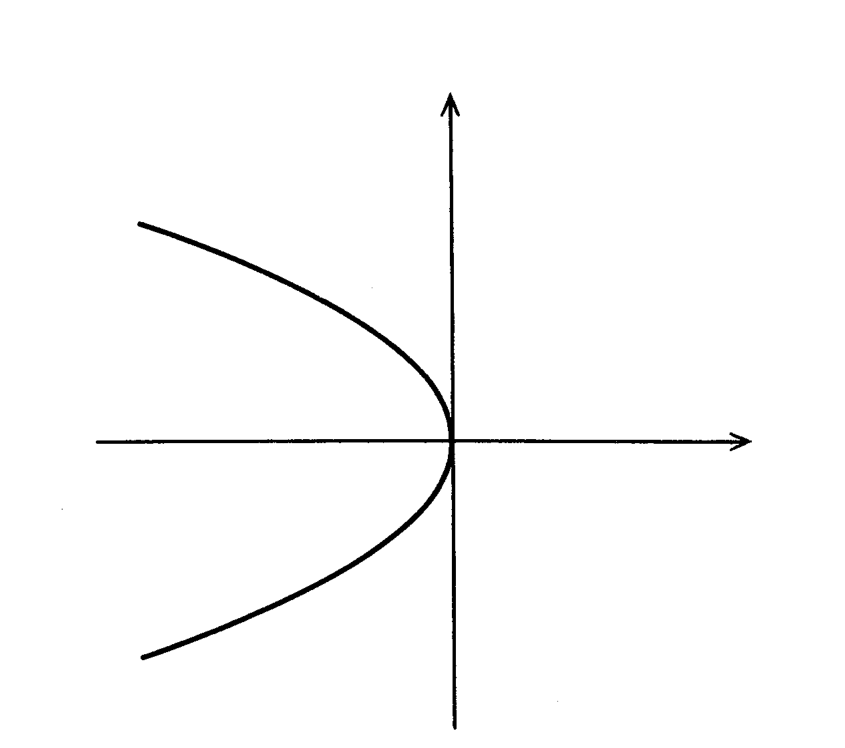
\includegraphics[width=0.45\textwidth]{figures/fig4.1.png}
  \figtitle{4.1}{$i_F$（原书 p.125）}
\end{figure}

\begin{example}{4.14}
  令 $n=2$，$m=1$，
  \[
    F(q_1,q_2,x)=x^4+2q_1x^2+4q_2x.
  \]
  $L_F$ 由方程 $x^3+q_1x+q_2=0$ 给出。取 $x=x$，$y=q_1$ 为 $L_F$ 的
% [原文 p.125]
  坐标。$i_F:L_F\to\R^4$ 由 $i_F(x,y)=(y,-x^3-xy,2x^2,4x)$ 给出。
\end{example}

例 4.14 是 4 维中的 2 维图形，所以图不能照原样画出。但是，按如下方式考虑，就能“看到”大致的形状。

讨论一般的拉格朗日浸入 $i:L\to T^*M$。考虑 $i$ 与 $\pi:T^*M\to M$ 的合成。

\begin{definition}{4.15}
  $p\in M$ 位于拉格朗日浸入 $i:L\to T^*M$ 的\textbf{焦点集}（caustics）上，是指存在 $x\in L$，使 $\pi i(x)=p$，且 $\rd_x\pi\circ i:T_xL\to T_pM$ 不可逆。

  当有拉格朗日子流形 $L\subset T^*M$ 时，映射 $\pi:L\to M$ 的奇点称为\textbf{拉格朗日奇点}（Lagrange singularity）。
\end{definition}
% [Tutor Note: 焦点集即光学中的焦散面：把 $L$ 投影到 $M$ 时，投影的临界值组成它。非焦点处的 $L$ 局部是一族闭 1-形式图像的并，这正是“多值闭 1-形式”的字面含义。]

说明焦点集的几何意义。为简单起见，设 $i$ 是嵌入。此时，若 $p\in M$ 不在焦点集上，且 $L$ 紧，则对 $p$ 附近的 $q$，$T_q^*M$ 与 $L$ 的交点数不依赖于 $q$。因此在 $p$ 附近存在微分 1-形式 $u_1,\dots,u_m$，$L$ 是它们图像之并。由推论 4.3，$u_i$ 是闭微分形式。也就是说，在焦点集之外，$L$ 可以看作多值闭微分 1-形式的图像。在焦点集附近则不然。知道了焦点集及其附近 $L$ 的样子，就知道了 $L$ 的大致样子。

例 4.14 的情形，$\pi\circ i_F(x,y)=(y,-x^3-xy)$。这个雅可比行列
% [原文 p.126]
式是 $3x^2+y$，因此焦点集以 $x$ 为参数是 $(-3x^2,2x^3)$。这由图 4.2 表示。注意原点是奇点（尖点）。图 4.2 的区域 1 中 $L$ 是 3 值微分 1-形式的图像，区域 2 中 $L$ 是 1 值微分 1-形式的图像。

\begin{figure}[htbp]
  \centering
  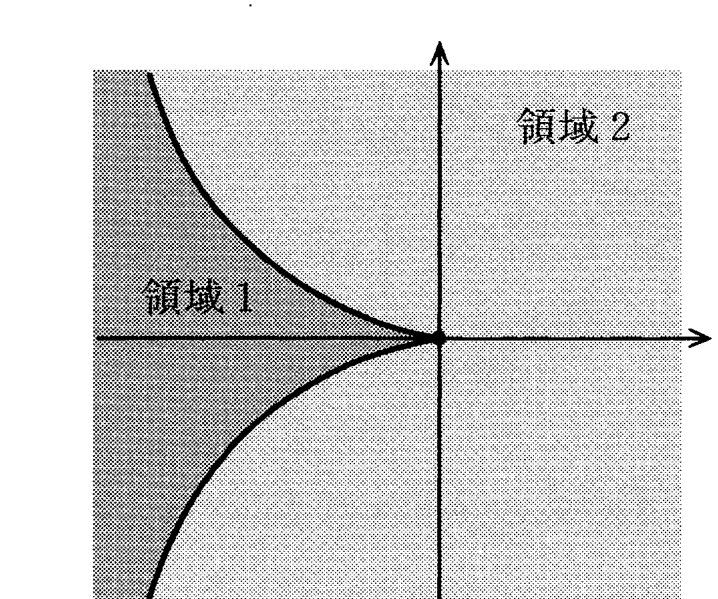
\includegraphics[width=0.42\textwidth]{figures/fig4.2.png}
  \figtitle{4.2}{尖点（原书 p.126）}
\end{figure}

\begin{theorem*}{4.16}
  对 $T^*\R^n$ 的任意拉格朗日子流形 $L$ 与 $x\in L$，存在 $\pi(x)$ 的邻域 $U$、$m\in\Z_+$ 以及 $U\times\R^m$ 上的函数 $F$，使 $F$ 满足 (4.1)，且 $L\cap T^*U=i_F(L_F)$。
\end{theorem*}
\begin{proof}
  设 $q_1,\dots,q_n,p_1,\dots,p_n$ 为 $T^*\R^n$ 的标准坐标。由于 $\omega(\frac{\partial}{\partial q_i},\frac{\partial}{\partial p_i})=1$，对每个 $i$，下列 (4.3)、(4.4) 之一成立：
  \begin{align}
    \frac{\partial}{\partial q_i}\notin T_xL \tag{4.3}\\
    \frac{\partial}{\partial p_i}\notin T_xL \tag{4.4}
  \end{align}
  必要时重排顺序，可设 $i=1,\dots,m$ 时 (4.3) 成立，$i=m+1,\dots,n$ 时 (4.4) 成立。令
  \[
    \Psi(q_1,\dots,q_n,p_1,\dots,p_n)=(p_1,\dots,p_m,q_{m+1},\dots,q_n,-q_1,\dots,-q_m,p_{m+1},\dots,p_n).
  \]
  $\Psi$ 是辛同胚。由于 $T_{\Psi(x)}\Psi(L)$ 与 $T^*\R^n$ 的纤维横截，在 $\Psi(x)$ 附近 $\Psi(L)$ 是微分 1-形式 $u$ 的图像。
% [Tutor Note: 这个 $\Psi$ 把 $q_i$ 与 $p_i$（$i\le m$）互换，相当于对这 $m$ 个方向作部分 Fourier 变换；(4.3) 保证这些方向上可以用 $p_i$ 当坐标，故 $\Psi(L)$ 在纤维方向投影为图像。]
% [原文 p.127]
  由推论 4.3，存在 $n$ 元函数 $S$ 使 $u=\rd S$。于是 $\Psi(L)$ 可表为
  \begin{equation}
    p_i=\frac{\partial S}{\partial q_i} \tag{4.5}
  \end{equation}
  在 $S$ 中代入变量 $p_1,\dots,p_m,q_{m+1},\dots,q_n$。则由 (4.5)，$L$ 在 $x$ 附近可表为
  \begin{equation}
    q_i=-\frac{\partial S}{\partial p_i},\quad i\le m \text{ 时} \tag{4.6}
  \end{equation}
  \begin{equation}
    p_i=+\frac{\partial S}{\partial q_i},\quad i>m \text{ 时}. \tag{4.7}
  \end{equation}
  现在取新变量 $\lambda_1,\dots,\lambda_m$，令
  \[
    F(q_1,\dots,q_n,\lambda_1,\dots,\lambda_m)=q_1\lambda_1+\dots+q_m\lambda_m+S(\lambda_1,\dots,\lambda_m,q_{m+1},\dots,q_n).
  \]
  于是 $L_F$ 由 $q_i=-\partial S/\partial\lambda_i$（$i=1,\dots,m$）表示。又
\[
  \resizebox{0.97\linewidth}{!}{$\begin{aligned} i_F(q_1,\dots,q_n,\lambda_1,\dots,\lambda_m) &=\left(q_1,\dots,q_n,\frac{\partial S}{\partial q_1},\dots,\frac{\partial S}{\partial q_m}\right)\\ &=\left(-\frac{\partial S}{\partial\lambda_1},\dots,-\frac{\partial S}{\partial\lambda_m},q_{m+1},\dots,q_n,\lambda_1,\dots,\lambda_m,\frac{\partial S}{\partial q_{m+1}},\dots,\frac{\partial S}{\partial q_n}\right). \end{aligned}$}
\]
  因此由 (4.6)、(4.7) 得 $i_F(L_F)=L$。
\end{proof}
% [Tutor Note: 原书 p.127 上式的第二行印作 $(q_1,\dots,q_n,\partial S/\partial q_1,\dots,\partial S/\partial q_m)$；按 $\partial F/\partial q_i=\lambda_i$（$i\le m$）应为 $(q_1,\dots,q_n,\lambda_1,\dots,\lambda_m,\partial S/\partial q_{m+1},\dots,\partial S/\partial q_n)$，方与下一行一致，疑为笔误。]

由命题 4.11、定理 4.16，余切丛的拉格朗日子流形的局部考察，归结为生成函数的考察。

生成函数的考察与可微映射奇点的研究如下联系起来。设 $F(\vec q,\vec\lambda)$ 为生成函数。不妨设 $(0,0)\in L_F$，即把 $F(0,\vec\lambda)$ 看作 $\vec\lambda$ 的函数时以 $0$ 为奇点。但由 (4.1)，$(0,0)$ 并不是把 $F$ 看作 $\vec q$、$\vec\lambda$ 两方函数时 $F$ 的奇点。

把 $F_{\vec q}(\vec\lambda)=F(\vec q,\vec\lambda)$ 看作以 $\vec\lambda$ 为变量的 $\R^m$ 上光滑映射的、以 $\vec q$ 为参数的族。也就是看作把以 $0$ 为奇点的函数加以形变所得之物。这样的东西称为奇点的\textbf{开析}（unfolding）。于是拉格朗日子流形的局部问题归结为研究奇点及其开析的问题。

% [原文 p.128]
Arnold 把焦点集的形状与奇点分类联系起来，在维数较低时进行了分类，并发现了它与 Dynkin 图（Dynkin diagram）及镜映变换群（reflection group）的关系（参照 [11], [14], [16] 等）。他进而由奇点分类发现了奇妙的双对性（strange duality）。这些被认为与镜像对称密切相关，但它们之间究竟如何相关，研究目前正在进行。

用函数族 $F_{\vec q}$ 的语言，焦点集可如下刻画。

\begin{lemma*}{4.17}
  $\vec q$ 位于 $i_F(L_F)$ 的焦点集上，等价于存在 $\vec\lambda_0$ 使 $\rd_{\vec\lambda_0}F_{\vec q}=0$ 且 $\det(\mathrm{Hess}_{\vec\lambda_0}F_{\vec q})=0$。$\mathrm{Hess}_{\vec\lambda_0}F_{\vec q}$ 指 Hessian 矩阵。
\end{lemma*}
\begin{proof}
  $\rd_{\vec\lambda_0}F_{\vec q}=0$ 与 $(\vec q,\vec\lambda_0)\in L_F$ 等价。在 $(\vec q,\vec\lambda_0)$ 处的 $m\times m$ 矩阵 $\left(\frac{\partial F}{\partial\lambda_i\partial\lambda_j}\right)$ 记为 $A$，$n\times m$ 矩阵 $\left(\frac{\partial F}{\partial\lambda_i\partial q_j}\right)$ 记为 $B$。按定义
  \[
    T_{(\vec q,\vec\lambda_0)}L_F=\{(\vec a,\vec b)\in\R^m\times\R^n\mid A\vec a+B\vec b=0\}
  \]
  可表出。又 $\rd\pi:T_{(\vec q,\vec\lambda_0)}L_F\to T_{\vec q}\R^n$ 为 $(\vec a,\vec b)\mapsto\vec b$。由假设，$(n+m)\times m$ 矩阵 $(A\ B)$ 的秩为 $m$，故 $\rd\pi$ 是同构与 $A$ 可逆等价。引理 4.17 由这一事实与定义立得。
\end{proof}
% [Tutor Note: 原书 p.128 这里 A、B 的分量印作一阶偏导 $\partial F/\partial\lambda_i\partial\lambda_j$ 等，且 B 记为 $n\times m$、$(A\ B)$ 记为 $(n+m)\times m$；按文意应为二阶偏导 $\partial^2F$，且 $B$ 应为 $m\times n$、$(A\ B)$ 应为 $m\times(n+m)$，否则 $A\vec a+B\vec b$ 的维数对不上。]

使 $\rd f=0$ 的所有点处 Hessian 矩阵都可逆的函数 $f$，就是 Morse 函数。Morse 函数即使稍作形变，也能通过坐标变换与原函数重合（Morse 引理，[248], [257], [274]）。此事称为 Morse 函数是\textbf{稳定的}（stable）。反之，已知若函数稳定则是 Morse 函数。引理 4.17 意味着焦点集与使 $F_{\vec q}$ 不稳定的所有 $\vec q$ 的集合一致。换言之，焦点集是发生突变（catastrophe）的点，即分岔（bifurcation）集。在突变理论的术语中，例 4.13 称为折叠（fold），例 4.14 称为尖点（cusp）。

以上关于生成函数只叙述了局部理论。应用生成函数研究余切丛的拉格朗日子流形的整体性质的工作，近年来兴盛起
% [原文 p.129]
来。拉格朗日子流形的整体研究，用伪全纯曲线的方法由 Gromov 与 Eliashberg 引入并取得进展；而 Viterbo 等人表明，用生成函数也能平行地导出许多结果。用生成函数的方法比用伪全纯曲线的方法初等，这是一大优点。参见 [143], [380] 等。

\section{接触流形与勒让德子流形}

\takeaway{接触结构是辛结构的奇数维类似物，由满足 $\theta\wedge(\rd\theta)^n\neq0$ 的接触形式确定。勒让德子流形是接触形式在其上为零的 $n$ 维子流形，它与拉格朗日子流形的关系由“辛化”$N\times\R$ 联系起来。}

\begin{definition}{4.18}
  $2n+1$ 维流形 $M$ 上的微分 1-形式 $\theta_M$ 称为\textbf{接触形式}（contact form），是指微分 $2n+1$-形式 $\theta_M\wedge\rd\theta_M^n$ 绝不消失。

  $2n+1$ 维流形 $M$ 的切丛 $TM$ 的秩 $n$ 子丛 $\xi\subset TM$ 称为\textbf{接触结构}（contact structure），是指对每点 $p\in M$，其邻域上存在接触形式 $\theta_M$，使 $\mathrm{Ker}\,\theta_M=\xi$ 在 $p$ 的邻域上成立。
\end{definition}

定义的条件 $\theta_M\wedge\rd\theta_M^n\neq0$，等价于 $\theta_M$ 不为 $0$、且 $\mathrm{Ker}\,\theta_M=\xi_M$ 上由 $\rd\theta_M$ 确定的反对称 2-次形式非退化。

当 $\mathrm{Ker}\,\theta_M=\xi_M$ 时，接触流形自然有定向。即：在 $\mathrm{Ker}\,\theta_M$ 上非退化 2-次形式 $\rd\theta_M$ 决定定向，在 $\mathrm{Ker}\,\theta_M$ 的补空间上 $\theta_M$ 决定定向。以下设接触流形带定向，且作为接触形式 $\theta_M$ 只考虑其所定定向与 $M$ 原有定向相容者。
% [Tutor Note: 这里“只取与定向相容的 $\theta_M$”是为了让 Reeb 向量场的符号约定（定义 4.22 的 $\theta_M(X_f)=-f$）不依赖于 $\theta_M$ 的符号；若把 $\theta_M$ 换成 $-\theta_M$，接触结构不变而 Reeb 场变号。]

接触结构是辛结构的奇数维类似物，出现在各种场合。从 Darboux 定理、Moser 定理的类似物开始吧。

\begin{theorem}{4.19}
  对 $M$ 上任一接触形式 $\theta_M$，在各点周围可取坐标系，使
  \[
    \theta_M=\rd q_0-p_1\rd q_1-\dots-p_n\rd q_n
  \]
  成立。$q_0,\dots,q_n,p_1,\dots,p_n$ 也称为 Darboux 坐标。
\end{theorem}

\begin{theorem}{4.20}
  $M$ 上接触形式以 $\tau$ 为参数的任意光滑族
% [原文 p.130]
  $\theta_\tau$，都存在微分同胚 $\varphi_\tau:M\to M$ 的光滑族，使 $\varphi_\tau^*\theta_\tau=\theta_0$，$\varphi_0=\id$。
\end{theorem}

下面叙述 Darboux 定理、Moser 定理的证明所依据的定理 2.18 的类似物。

\begin{definition}{4.21}
  $\varphi:(M,\xi_M)\to(N,\xi_N)$ 称为\textbf{接触同胚}（contact diffeomorphism），是指保持定向的微分同胚，且 $\varphi_*\xi_M=\xi_N$。当 $M=N$ 时称为\textbf{接触变换}（contact transform）。$\mathrm{Aut}(M,\xi_M)$ 指接触变换全体构成的李群。
\end{definition}

当 $\xi_M=\mathrm{Ker}\,\theta_M$ 时，这等价于存在 $h\in C^\infty(M)$、$h>0$，使 $\varphi^*\theta_M=h\theta_M$。

当 $\xi_M=\mathrm{Ker}\,\theta_M$ 时，$\mathrm{Aut}(M,\xi_M)$ 也写作 $\mathrm{Aut}(M,\theta_M)$。

计算 $\mathrm{Aut}(M,\xi_M)$ 的李代数。下面的定义中固定 $\theta_M$。

\begin{definition}{4.22}
  对 $M$ 上的函数 $f$，用如下条件定义 $f$ 生成的\textbf{哈密顿向量场} $X_f$：
  \begin{enumerate}
    \item 对任意 $V\in\xi_M$，$\rd f(V)=(\rd\theta_M)(X_f,V)$ 成立；
    \item $\theta_M(X_f)=-f$。
  \end{enumerate}
  由这两个条件，$X_f$ 唯一确定，这从接触结构的定义可以明白。
\end{definition}

在 Darboux 坐标中，$X_f$ 由下式给出：
\[
  X_f=\left(-f+\sum p_i\frac{\partial f}{\partial p_i}\right)\frac{\partial}{\partial q_0}-\sum\left(\frac{\partial f}{\partial q_i}+p_i\frac{\partial f}{\partial q_0}\right)\frac{\partial}{\partial p_i}+\sum\frac{\partial f}{\partial p_i}\frac{\partial}{\partial q_i}.
\]
% [Tutor Note: 验证 (1) 时注意 $V\in\xi_M$ 有分量 $V=\sum v_i\partial_{q_i}+\dots$ 且 $v_0=\sum p_iv_i$；(2) 中 $\theta_M(X_f)=-f$ 与 $\theta_M(\partial_{q_0})=1$ 联立即得上式头一项的 $-f$。]

\begin{lemma*}{4.23}
  $\mathrm{Aut}(M,\theta_M)$ 的李代数与哈密顿向量场 $X_f$ 全体一致。
\end{lemma*}
\begin{proof}
  $\mathrm{Aut}(M,\theta_M)$ 的李代数与使 $L_X\theta_M=h\theta_M$ 的 $h$ 存在的 $X$ 全体一致。由 (2.8) 与 $X_f$ 的定义，在 $\xi_M$ 上
  \[
    L_{X_f}\theta_M=(\rd\circ i_{X_f}+i_{X_f}\circ\rd)\theta_M=0.
  \]
  故 $L_{X_f}\theta_M=h\theta_M$。反之设 $L_X\theta_M=h\theta_M$。令 $f=-\theta_M(X)$。由 (2.6)，在 $\xi_M$ 上 $0=\rd f+i_X(\rd\theta_M)$。因此 $X=X_f$。
\end{proof}

% [原文 p.131]
用引理 4.23，定理 4.19、4.20 可与 Darboux 定理、Moser 定理同样地证明（留给读者）。

\begin{definition}{4.24}
  当 $f\equiv-1$ 时的 $X_f=X_{-1}$ 称为\textbf{Reeb 向量场}（Reeb vector field）。
\end{definition}

$T_pM$ 由 $\xi_M$ 与 $X_{-1}$ 张成，且 $(\rd\theta_M)(X_{-1},X_{-1})=0$。因此 $i_{X_{-1}}(\rd\theta_M)=0$ 成立。在 Darboux 坐标中 $i_{X_{-1}}=\partial/\partial q_0$。
% [Tutor Note: 原书 p.131 这一句把向量场与内乘混写；Darboux 坐标下应为 $X_{-1}=\partial/\partial q_0$，而 $i_{X_{-1}}$ 是缩并算子。]

下面的猜想是接触几何的基本问题。

\begin{conjecture}{4.25}
  （Weinstein 猜想）$H^1(M;\R)=0$ 的接触流形 $M$ 的 Reeb 向量场具有周期轨道。
\end{conjecture}

作为部分解，已知：$\C^n$ 的凸区域情形（Weinstein [38]）、$\C^n$ 星形区域边界的情形（Rabinowitz [311]）、$\C^n$ 的接触型子流形（定义 4.40）情形（Viterbo [378]）、同胚于 $S^3$ 的情形（Hofer [181]）等。

用 $X_{-1}$ 可以表示使 $L_{X_f}\theta_M=h\theta_M$ 的 $h$。

\begin{lemma*}{4.26}
  (1) $(\rd\theta_M)(X_f,X_{-1})=0$。

  (2) $L_{X_f}\theta_M=X_{-1}(f)\theta_M$。
\end{lemma*}
\begin{proof}
  因 $X_f+fX_{-1}$ 属于 $\xi_M$，由定义 4.22 的 (1) 得
  \[
    (\rd\theta_M)(X_f,X_{-1})=-(f\theta_M)(X_{-1},X_{-1})=0.
  \]
  (2) $L_{X_f}\theta_M=h\theta_M$ 中的 $h$ 的存在性已由引理 4.23 表明。而用 (1) 得
\[
  \resizebox{0.97\linewidth}{!}{$\displaystyle h=(L_{X_f}\theta_M)(X_{-1})=(i_{X_f}\rd+\rd i_{X_f})(\theta_M)(X_{-1})=(\rd\theta_M)(X_f,X_{-1})+(\rd f)(X_{-1})=X_{-1}(f). $}
\]
\end{proof}

\begin{definition}{4.27}
  对接触流形，\textbf{泊松括号} $\{f,g\}$ 定义为
  \[
    \{f,g\}=X_g(f)-fX_{-1}(g).
  \]
\end{definition}

\begin{theorem*}{4.28}
  $\{\cdot,\cdot\}$ 在 $C^\infty(M)$ 上确定李代数结构。$f\mapsto X_f$ 确定李代数同构 $(C^\infty(M),\{\cdot,\cdot\})\to\mathrm{Lie}(\Aut(M,\theta_M))$。
\end{theorem*}
\begin{proof}
  $f\mapsto X_f$ 确定向量空间同构 $(C^\infty(M),\{\cdot,\cdot\})\to\mathrm{Lie}(\Aut(M,\theta_M))$，这由引理 4.23 可知。注意 $L_XY=[Y,X]$ 进行计算，得
% [原文 p.132]
\[
  \resizebox{0.97\linewidth}{!}{$\displaystyle i_{[X_f,X_g]}\theta_M=(L_{X_g}i_{X_f}-i_{X_f}L_{X_g})\theta_M=-X_g(f)-i_{X_f}(X_{-1}(g)\theta_M)=-X_g(f)+X_{-1}(g)f=-\{f,g\}. $}
\]
  $[X_f,X_g]=X_h$ 的 $h$ 的存在由引理 4.23 得出。因此 $h=-i_{[X_f,X_g]}\theta_M=\{f,g\}$。也就是说，$f\mapsto X_f$ 保持括号积。特别地，$(M,\{\cdot,\cdot\})$ 是李代数。
\end{proof}

下面举接触流形的例子。都是重要的例子，关联的数学很丰富。首先考虑 $T^*M\times\R$。把 $\R$ 的坐标记为 $z$。

\begin{lemma*}{4.29}
  $\rd z-\theta$ 是 $T^*M\times\R$ 上的接触 1-形式。
\end{lemma*}
\begin{proof}
  $(\rd z-\theta)\wedge\rd(\rd z-\theta)^n=(-1)^n\rd z\wedge\rd\theta^n$。$\rd\theta^n$ 在 $T^*M$ 上决不消失，故 $(\rd z-\theta)\wedge\rd(\rd z-\theta)^n$ 决不消失。
\end{proof}

想推广引理 4.29 的构成。设 $(M,\omega_M)$ 为辛流形，并假设 $[\omega_M]\in H^2(M;\R)$ 含于 $H^2(M;\Z)$ 的像中。于是存在 $M$ 上的复线丛（$U(1)$ 丛）$\mathcal L$ 及其上的 $U(1)$ 联络 $\nabla$，其曲率 $F_\nabla$ 满足
\begin{equation}
  F_\nabla=2\pi\sqrt{-1}\,\omega. \tag{4.8}
\end{equation}
特别地 $c_1(\mathcal L)=[\omega]$。（例如参照 [205]。）

\begin{definition}{4.30}
  $(\mathcal L,\nabla)$ 称为\textbf{前量子化丛}（prequantization bundle）。
\end{definition}

前量子化将在下一节叙述。

把与 $\mathcal L$ 相伴的主 $U(1)=S^1$ 丛（的全空间）记作 $S(\mathcal L)$。$U(1)$ 的李代数为 $u(1)=\sqrt{-1}\R$，故 $\nabla$ 的联络形式 $\theta$ 是 $S(\mathcal L)$ 上的 $u(1)$ 值微分 1-形式。由 $\R\cong u(1)$、$t\mapsto2\pi\sqrt{-1}t$ 确定，$\theta$ 可看作普通的微分 1-形式。由 (4.8) 与联络形式、曲率的定义可知 $\rd\theta=\pi^*\omega$。

\begin{lemma*}{4.31}
  $\theta$ 是 $S(\mathcal L)$ 上的接触 1-形式。
\end{lemma*}
\begin{proof}
  由 $\rd\theta=\pi^*\omega$，$\theta\wedge\rd\theta^n=\theta\wedge\pi^*\omega^n$。$\omega^n$ 是 $M$ 上决不消失的 $2n$ 次形式，且 $\theta$ 在纤维 $S^1$ 上的限制仍不为 $0$，故 $\theta\wedge\rd\theta^n$ 决不消失。
\end{proof}

由定义可以明白，$S(\mathcal L)$ 的 Reeb 向量场的轨道是 $S(\mathcal L)\to M$
% [原文 p.133]
的纤维。

举另一类例子。设 $(M,J_M)$ 为 $n$ 维复流形。$N$ 为 $M$ 的带定向的实 $2n-1$ 维子流形（超曲面）。令
\begin{equation}
  \xi_N=\{V\in TN\mid J_M(V)\in TN\}. \tag{4.9}
\end{equation}
$\xi_N$ 是 $TN$ 的秩 $2n-2$ 的子丛。$\pi:TN\to TN/\xi_N$ 为射影。

\begin{lemma*}{4.32}
  （秩 1 的实）向量丛 $TN/\xi_N$ 是平凡的。
\end{lemma*}
\begin{proof}
  $\xi_N$ 是复向量丛，故带定向。$TN$ 由假设带定向。因此 $TN/\xi_N$ 带定向。故作为秩 1 的实向量丛，它是平凡的。
\end{proof}

以下在 $TN/\xi_N$ 上选一个平凡化（因 $TN$、$\xi_N$ 带定向，选与此定向相容的平凡化）。对 $\xi_N$ 的截面 $V_1,V_2$，令
\[
  L(V_1,V_2)=\pi([V_1,J_MV_2]).
\]
由于已定 $TN/\xi_N$ 的平凡化，右边成为函数。

\begin{lemma*}{4.33}
  (1) $L(fV_1,V_2)=L(V_1,fV_2)=fL(V_1,V_2)$，

  (2) $L(V_1,V_2)=L(V_2,V_1)$，

  (3) $L(J_MV_1,J_MV_2)=L(V_1,V_2)$。
\end{lemma*}
\begin{proof}
  $\pi([fV_1,V_2])=\pi(f[V_1,V_2]-V_2(f)V_1)$。因 $\pi(V_1)=0$，(1) 成立。因 $J_M$ 可积，$[J_MV_1,J_MV_2]=J_M[V_1,V_2]$。由此得 (2)、(3)。
\end{proof}

由引理 4.33，$L$ 是 $\xi_N$ 上的对称 2-次形式。

\begin{definition}{4.34}
  $L$ 称为\textbf{Levi 形式}（Levi form）。当 Levi 形式正定时，带定向超曲面 $N$ 称为\textbf{拟凸}（pseudo convex）的。
\end{definition}

\begin{remark}{4.35}
  确定 $N$ 的定向后，$TN/\xi_N$ 的定向就确定了，因此 Levi 形式正定这一条件不依赖于（与此定向相容的）$TN/\xi_N$ 的平凡化。
\end{remark}

\begin{lemma*}{4.36}
  若 $H$ 非退化，则 $\xi_N$ 是接触结构。
\end{lemma*}
% [Tutor Note: 原书 p.133 的这条条件写作 $H$，但 $H$ 未在别处定义；按证明中 $(\rd\theta_N)(V_1,V_2)=L(V_1,J_MV_2)$ 的关系，所需的假设是“$L$ 非退化”，$H$ 疑为 $L$ 之误。]
\begin{proof}
% [原文 p.134]
  把 $TN\to TN/\xi_N\to\R$ 看作 $TN^*$ 的截面，即 $N$ 上的微分 1-形式。记之为 $\theta_N$。$\mathrm{Ker}\,\theta_N=\xi_N$ 是显然的，故只需证明 $\theta_N$ 是接触形式。为此只需证明在 $\mathrm{Ker}\,\theta_N$ 上 $\rd\theta_N$ 非退化。设 $V_1,V_2$ 为 $\xi_N$ 的截面，则
  \[
    (\rd\theta_N)(V_1,V_2)=V_1\theta_N(V_2)-V_2\theta_N(V_1)-\theta_N[V_1,V_2]=L(V_1,J_MV_2),
  \]
  故由假设，在 $\xi_N$ 上 $\rd\theta_N$ 非退化。
\end{proof}

$\C^n$ 的具有光滑边界的区域 $U$ 称为拟凸的，是指其边界 $\partial U$ 的 Levi 形式非退化。对任意拟凸区域 $U$，存在在 $U$ 上定义的全纯函数，它不能作为全纯函数解析延拓到 $U$ 之外。这称为 Levi 问题，由岡潔解决（参照 [297] 等）。

说明拟凸性的判定法。拟凸性是局部条件，故在各点 $p\in N$ 的邻域考虑即可。取 $p$ 附近 $M$ 的复坐标 $z_1,\dots,z_n$，设 $N$ 在 $p$ 附近由函数 $h$ 表为 $h(z_1,\dots,z_n)=0$。矩阵
\[
  \left(\frac{\partial^2h}{\partial z_i\partial\bar z_j}\right)
\]
称为 Levi 矩阵。

\begin{lemma}{4.37}
  $N$ 拟凸的充要条件是 Levi 矩阵正定。
\end{lemma}

证明见多变量复函数论的书，例如 [297]。

由引理 4.36 构造的接触流形，用 CR 结构（Cauchy–Riemann 结构，Cauchy-Riemann structure）来研究。CR 结构参见 [35] 等。

\begin{example}{4.38}
  设 $f_1,\dots,f_m$ 为 $\C^n$ 的 $0$ 的邻域上定义的全纯函数。令
  \[
    X=\{(z_1,\dots,z_n)\mid f_1(z_1,\dots,z_n)=\dots=f_m(z_1,\dots,z_n)=0\}.
  \]
  假设除 $0$ 外 $X$ 无奇点。此时，对充分小的 $\epsilon$，令
  \[
    X(\epsilon)=\{(z_1,\dots,z_n)\in X\mid \textstyle\sum|z_i|^2=\epsilon\}.
  \]
  $X(\epsilon)$ 是拟凸的（证明用引理 4.37 即可）。因此 $X(\epsilon)$ 是接触流形。
\end{example}

% [原文 p.135]
例 4.38 中重要的是 $f_i$ 为多项式且为加权齐次（weighted homogeneous）的情形。即，令 $\deg(z_j)=k_j$，
\[
  f_i=\sum_\ell c_\ell z_1^{m_{1,\ell}}\cdots z_n^{m_{n,\ell}}
\]
时，各项的权 $k_1m_{1,\ell}+\dots+k_nm_{n,\ell}$ 不随 $\ell$ 而变的情形。此时取
\[
  S(\epsilon)=\{(z_1,\dots,z_n)\in\C^n\mid \textstyle\sum|z_i|^{2k_i}=\epsilon\},
\]
并考虑 $X(\epsilon)=S(\epsilon)\cap X$ 更自然。$X(\epsilon)$ 仍然是拟凸的。
% [Tutor Note: 原书 p.135 此处把集合写成“$(z_1,\dots,z_n)\in\sum|z_i|^{2k_i}=\epsilon$”，脱漏了定义域与分隔竖线，译文按文意补足为 $\C^n$ 与“$|$”。]

\begin{lemma*}{4.39}
  $X(\epsilon)$ 的 Reeb 向量场全部是周期的（即积分曲线全部闭合为 $S^1$）。
\end{lemma*}
\begin{proof}
  考虑 $\C^n$ 上的函数 $f(z_1,\dots,z_n)=\sum|z_i|^{2k_i}$。由 $f$ 生成的哈密顿向量场的 1 参数变换群由
  \[
    \varphi_\tau(z_1,\dots,z_n)=(\exp(2\pi\sqrt{-1}\tau k_1)z_1,\dots,\exp(2\pi\sqrt{-1}\tau k_n)z_n)
  \]
  给出。由定义，$\varphi_\tau$ 保持 $X(\epsilon)$ 不变。$\varphi_\tau$ 是 Reeb 向量场的积分曲线，这可由简单计算验证。
\end{proof}

以上叙述了复流形的超曲面成为接触流形的情形。下面考虑 $(M,\omega_M)$ 为 $2n$ 维辛流形、$N$ 为其（带定向的）超曲面的情形。

\begin{definition}{4.40}
  $N$ 称为\textbf{接触型子流形}（submanifold of contact type），是指 $N$ 上存在接触形式 $\theta_N$，使 $N$ 满足 $\rd\theta_N=-\omega_M$。
\end{definition}

接触型辛子流形的重要例子是（余）球面束。设 $M$ 为黎曼流形，
\begin{equation}
  S(M)=\{(q,v)\in TM\mid \|v\|=1\}. \tag{4.10}
\end{equation}
在 $S(M)$ 上定义接触形式。首先，用黎曼度量可确定切空间与余切空间之间的同构（此等同也称为勒让德变换）。因此也可以看作
\[
  S(M)=S^*(M)=\{(q,v)\in T^*M\mid \|v\|=1\}.
\]
称 $S^*(M)$ 为\textbf{余切球面束}。

\begin{lemma*}{4.41}
  基本 1-形式 $\theta$ 的限制是 $S(M)$ 的接触形式。特别地，$S(M)$ 是接触型子流形。
\end{lemma*}
\begin{proof}
% [原文 p.136]
  在余切丛中考虑。由 $f:T^*M\to\R$、$f(p,v)=g_M(v,v)$ 定义 $f$。考虑其哈密顿向量场 $X_f$。因 $S(M)=f^{-1}(1)$ 且 $X_f(f)=0$，故 $X_f$ 与 $S(M)$ 相切。设 $V\in TS^*(M)$，则
  \begin{equation}
    \omega_{T^*M}(X_f,V)=\rd f(V)=V(f)=0. \tag{4.11}
  \end{equation}
  另一方面，$\theta(X_f)=2$ 容易验证。因此 $\mathrm{Ker}\,\theta$ 不含 $X_f$。又 $\omega_{T^*M}=-\rd\theta$ 到 $TS^*(M)$ 的限制的秩为 $2n-2$。因此由 $\theta(X_f)=2$，$\rd\theta$ 在 $\mathrm{Ker}\,\theta$ 上非退化。
\end{proof}

在 凯勒流形情形，拟凸与接触型相似但有不同（见 [95]）。

以上叙述的是辛流形的子流形上带有接触流形结构的情形，此外还有反方向的构成。设 $N$ 为接触流形，$\theta_N$ 为其接触形式。用
\[
  \omega=e^\tau(\rd\theta_N+\rd\tau\wedge\theta_N)
\]
定义 $N\times\R$ 上的微分 2-形式 $\omega$。这里 $\tau$ 是 $\R$ 的坐标。

\begin{lemma}{4.42}
  $(N\times\R,\omega)$ 是辛流形。
\end{lemma}

证明是简单的计算。

\begin{definition}{4.43}
  $(N\times\R,\omega)$ 称为接触流形 $(N,\theta_N)$ 的\textbf{辛化}（symplectization）。
\end{definition}

辛化被 Hofer 等人用于 Weinstein 猜想的研究与接触同调（contact homology）（参照 [181], [94]）。

\begin{remark}{4.44}
  考虑接触流形 $(N,\xi_N)$，在 $\xi_N$ 上取度量。对 $p,q\in N$，考虑连接 $p$ 与 $q$、且在每点与 $\xi_N$ 相切的路径，其长度的下确界记为 $d(p,q)$。已知 $d(p,q)$ 使 $N$ 成为距离空间。此距离称为 \textbf{Carnot–Carathéodory 距离}（Carnot-Carathéodory metric），其几何称为\textbf{次黎曼几何}（sub Riemannian geometry）。（考虑 Carnot–Carathéodory 距离所需的 $\xi_N$ 的条件可比接触结构稍宽，称为 Hörmander 条件（Hörmander condition）。）这些最近被活跃地研究。其微分几何侧面见 [41]（及其中引用的文献）。此外，与次椭圆型微分方程（hypoelliptic differential equation）的关系（见 [178], [332] 等。Hörmander 条件的定义也见这些文献）、与控制理论（control theory）的关系（见 [188]§9.7, [4] 等）很重要。
\end{remark}
% [Tutor Note: 次黎曼几何中只允许沿 $\xi_N$ 方向运动，故两点间的“距离”可以远大于普通黎曼距离；若 $\xi_N$ 满足 Hörmander 条件（其李括号生成整个切丛），则 $d$ 仍给出与流形拓扑相容的度量。]

% [原文 p.137]
对接触流形，定义与辛流形的拉格朗日子流形相当的概念。设 $\theta_N$ 为 $2n+1$ 维流形 $N$ 上的接触形式。

\begin{definition}{4.45}
  $N$ 的 $n$ 维子流形 $L$ 称为\textbf{勒让德子流形}（Legendrian submanifold），是指 $\theta_N|_L=0$。勒让德浸入也类似地定义。
\end{definition}

勒让德子流形这一概念由接触结构决定，不依赖于接触形式的取法。

\begin{lemma*}{4.46}
  设 $L$ 为 $2n+1$ 维流形 $N$ 的子流形，$\theta_N$ 为 $N$ 上的接触形式，且 $\theta_N|_L=0$。则 $\dim L\le n$。
\end{lemma*}
\begin{proof}
  设 $p\in L$。由 $\theta_N|_L=0$，$T_pL$ 含于 $\xi_N$，且 $T_pL$ 上 $\rd\theta_N=0$。$\xi_N$ 上 $\rd\theta_N$ 确定非退化的反对称 2-次形式。因此把反对称 2-次形式化为标准形，即可容易地证明 $\dim L\le n$。
\end{proof}

举勒让德子流形的例子。

\begin{example}{4.47}
  $T_Y^*N\cap S^*(N)$ 是引理 4.41 的接触流形 $S^*(N)$ 的勒让德子流形。这一事实已在引理 4.4 的证明中表明。
\end{example}

\begin{lemma*}{4.48}
  在例 4.38 中设 $f_i$ 为实系数多项式。此时 $X(\epsilon)\cap\R^n$ 是 $X(\epsilon)$ 的勒让德子流形。
\end{lemma*}
\begin{proof}
  设 $p\in X(\epsilon)\cap\R^n$，$V\in T_p(X(\epsilon)\cap\R^n)$。设 $S^{2n-1}$ 为 $\C^n$ 的单位球面，则容易看出 $J(T_p\R^n\cap T_pS^{2n-1})\subset T_pS^{2n-1}$。因此 $JV\in T_pX(\epsilon)$。因 $V,JV\in T_pX(\epsilon)$，由定义得 $\theta_N(V)=0$。
\end{proof}

§4.1 中用生成函数说明了构造拉格朗日子流形的方法，其构造法实际上是在构造勒让德子流形。设 $V\to M$ 为向量丛，$F:V\to\R$ 为光滑函数。按 §4.1 定义 $L_F$。定义 $i_F^+:L_F\to T^*M\times\R$ 为 $i_F^+(q,\lambda)=(i_F(q,\lambda),F(q,\lambda))$（$i_F$ 如 §4.1）。

\begin{proposition*}{4.49}
  $i_F^+$ 是勒让德浸入。
\end{proposition*}
\begin{proof}
  用命题 4.11 的证明中的记号。$\R$ 的坐标记为 $z$。$\theta=\rd z-p_1\rd q_1-\dots-p_n\rd q_n$。因此
% [原文 p.138]
  \[
    i_F^{+*}\theta=\rd F-\sum_{i,j}\frac{\partial F}{\partial q_i}\frac{\partial q_i}{\partial y_j}\rd y_j=\rd F-\sum_j\frac{\partial F}{\partial y_j}\rd y_j=0.
  \]
\end{proof}

\begin{remark}{4.50}
  设 $\pi:T^*M\times\R\to T^*M$ 为射影。若有勒让德浸入 $i:L\to T^*M\times\R$，且合成 $\pi\circ i:L\to M$ 是浸入，则 $\pi\circ i$ 是拉格朗日浸入。此时，$\pi\circ i$ 称为到辛流形 $T^*M$ 的\textbf{完全拉格朗日浸入}（exact Lagrangian immersion）。$T^*M$ 的完全拉格朗日子流形也同理。
\end{remark}

用生成函数作出的拉格朗日浸入是完全拉格朗日浸入。用生成函数不能整体地表示的拉格朗日浸入之例，可用下面的命题作出。

\begin{proposition*}{4.51}
  设 $i^+:L\to T^*M\times\R$ 为勒让德浸入，$i=\pi\circ i^+:L\to T^*M$。则对任意 $\gamma\in\pi_1(L)$，
  \begin{equation}
    \int_\gamma i^*\theta=0 \tag{4.12}
  \end{equation}
  成立。反之，若拉格朗日浸入 $i:L\to T^*M$ 对任意 $\gamma\in\pi_1(L)$ 满足 (4.12)，则它是完全的。
\end{proposition*}
\begin{proof}
  由假设 $\int_\gamma i^{+*}(\rd z-\theta)=0$。另一方面 $\rd z$ 是恰当形式，故 $\int_\gamma i^{+*}\rd z=0$，因此 (4.12) 成立。

  反之，设 (4.12) 成立。固定 $x_0\in L$，对 $x\in L$ 取连接 $x_0$ 与 $x$ 的道路 $\ell_x$，令 $j(x)=\int_{\ell_x}i^*\theta$。由 (4.12)，右边的积分不依赖 $\ell_x$ 的取法。令 $i^+(x)=(i(x),j(x))$，由 $j$ 的定义可知 $i^+$ 是勒让德浸入。
\end{proof}
% [Tutor Note: (4.12) 说的是 $i^*\theta$ 在 $L$ 上零上同调，即 $i^*\theta=\rd j$ 整体可解；证明中把 $j$ 定义为沿道路的积分，正是这一原函数。$T^*M$ 中“完全”一词即指 $\theta$ 的拉回恰当。]
% [Tutor Note: 生成函数给出的 $i_F$ 满足 $i_F^*\theta=\rd F$（见命题 4.49 的证明），故必是完全拉格朗日浸入；例 4.52 将给出一个只在面积条件满足时才完全的环。]

\begin{figure}[htbp]
  \centering
  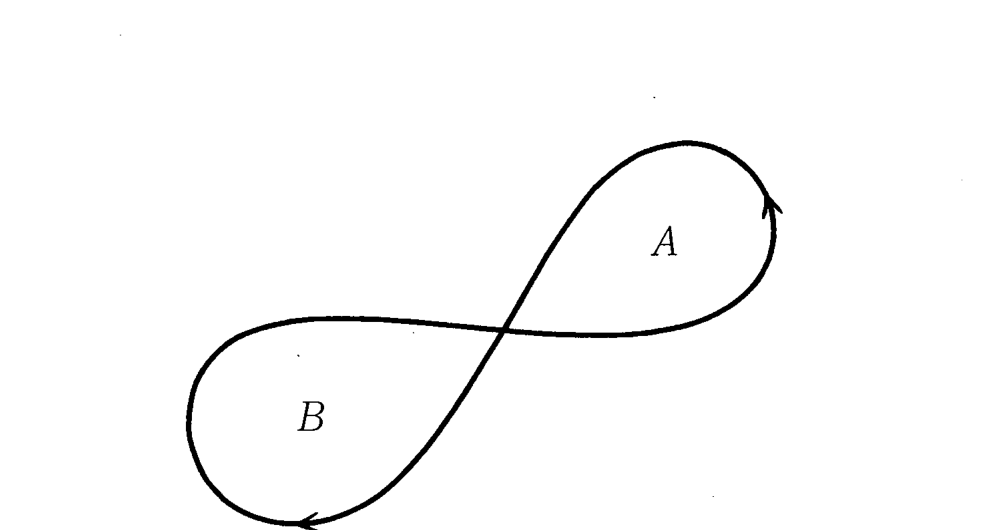
\includegraphics[width=0.62\textwidth]{figures/fig4.3.png}
  \figtitle{4.3}{拉格朗日子流形成为完全的条件（原书 p.139）}
\end{figure}

\begin{example}{4.52}
  设 $\R^2=T^*\R$，$i:S^1\to\R^2$ 为图 4.3 所表示的浸入。$\R^2$ 的所有 1 维子流形都是拉格朗日子流形，故 $i$ 是拉格朗日浸入。$i$ 成为完全拉格朗日浸入，是在图 4.3 的两个面积 $A$ 与 $B$ 一致之时。要看这一点，计算以 $\gamma\in\pi_1(S^1)$ 为生成元时的 $\int_\gamma\theta$ 即可（命题 4.51）。由 Stokes 定理与
% [原文 p.139]
  $\rd\theta=\omega$，这个数是 $A-B$。
\end{example}

\begin{definition}{4.53}
  设 $i^+:L\to T^*M\times\R$ 为勒让德浸入。设 $\pi:T^*M\times\R\to M\times\R$ 为射影。合成 $\pi\circ i^+:L\to M\times\R$ 称为\textbf{波前}（wave front）\footnote{超函数的 wave front 这一概念（佐藤幹夫）用于超局所解析。它与定义 4.53 有关系，但意义多少不同。}。又此映射的奇点称为\textbf{勒让德奇点}（Legendrian singularity）。
\end{definition}

\begin{example}{4.54}
  计算例 4.13 的情形，得 $\pi\circ i^+(x)=(-x^2,x^3-3x^5)$。同样在 $x=0$ 处有奇点。
\end{example}
% [Tutor Note: 原书 p.139 这里作 $(-x^2,\,x^3-3x^5)$；但由例 4.13，$F=x^3+3qx$ 在 $L_F$（$q=-x^2$）上等于 $-2x^3$，故正确的波前应为 $(-x^2,\,-2x^3)$，疑为笔误。]

\begin{example}{4.55}
  例 4.14 的情形是 $\pi\circ i^+(x,y)=(y,-x^3-xy,-3x^4-2x^2y)$（图 4.4）。
\end{example}

\begin{figure}[htbp]
  \centering
  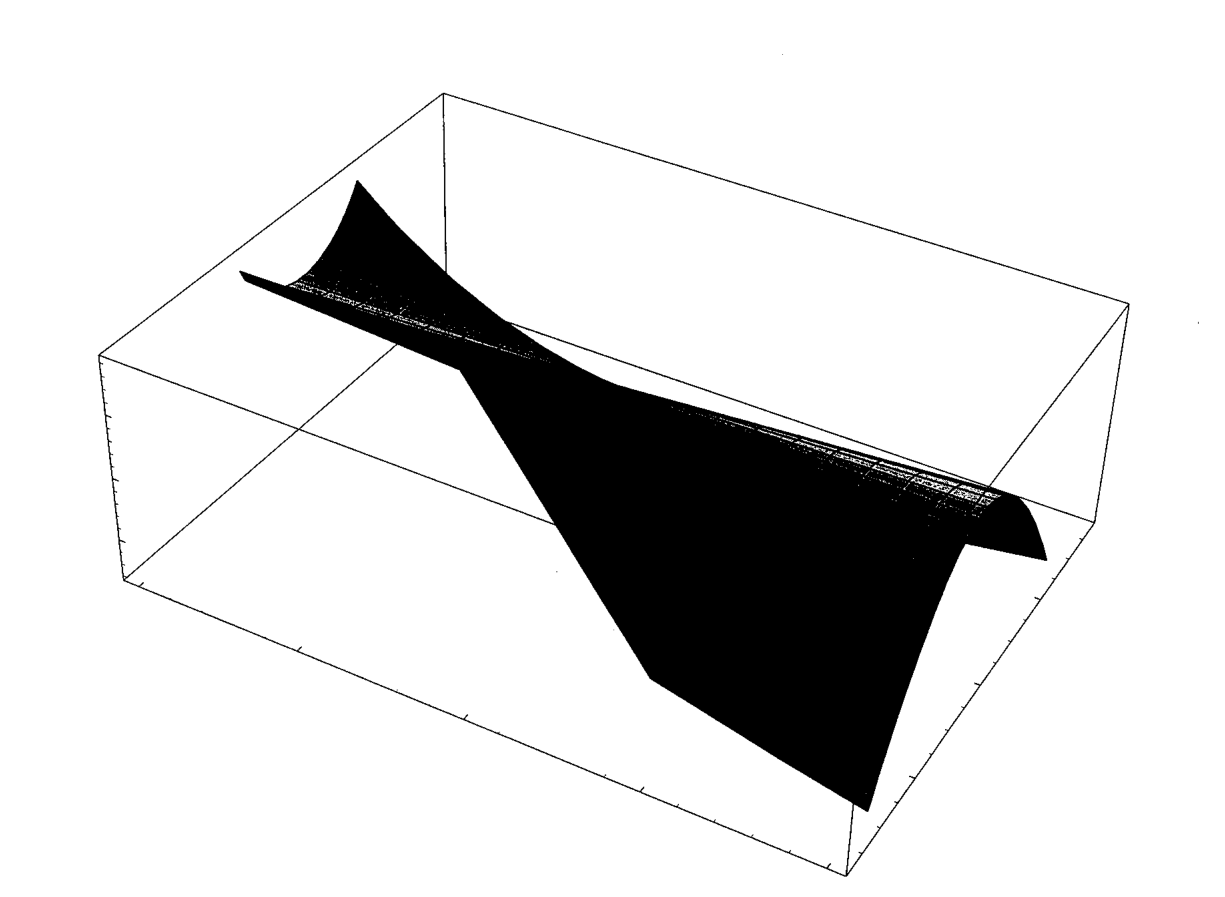
\includegraphics[width=0.62\textwidth]{figures/fig4.4.png}
  \figtitle{4.4}{波前的例子（原书 p.139）}
\end{figure}

% [原文 p.140]
只稍微谈一点勒让德奇点与黎曼几何、几何光学（geometric optics）的关系（详见 [165] 等）。设 $(M,g_M)$ 为黎曼流形。在余切丛 $T^*M$ 上定义函数 $f(p,v)=g_M(v,v)$。考虑由 $f$ 确定的哈密顿向量场 $X_f$。单位余切球面束 $S^*(M)$ 由 $f=1$ 表示，故被 $X_f$ 保持。即它确定了 $S^*(M)$ 上的向量场。$X_f$ 称为\textbf{测地流}（geodesic flow）。

\begin{lemma}{4.56}
  测地流是关于引理 4.41 的接触结构的 Reeb 向量场。
\end{lemma}

证明其实已在引理 4.41 的证明中完成。把 $X_f$ 生成的 1 参数变换群记为 $\varphi_\tau$。$\tau\mapsto\pi(\varphi_\tau(p)):\R\to M$ 是 $M$ 的测地线。

由引理 4.23、4.56，$\varphi_\tau^*\theta=\theta$ 成立。因此特别地，$\varphi_\tau$ 把勒让德子流形移到勒让德子流形。

设 $N$ 为 $M$ 的子流形，$T_N^*M\subset T^*M$ 为其余法丛。如例 4.47 所述，$S_N^*M$ 是勒让德子流形。因此 $\varphi_\tau(S_N^*M)$ 也是勒让德子流形。

\begin{definition}{4.57}
  $p\in M$ 是 $N$ 的\textbf{共轭点}（conjugate point），是指存在 $\tau$，使 $p=\pi(x)$、$x\in\varphi_\tau(S_N^*M)$，且 $\rd\pi:T_x\varphi_\tau(S_N^*M)\to T_pM$ 不是单射。
\end{definition}

换言之，共轭点是指对某个 $\tau$ 成为 $\varphi_\tau(S_N^*M)$ 的勒让德奇点的 $M$ 的点。

下面的引理可由定义容易地证明。考虑关于黎曼度量 $g_M$ 的指数映射 $\exp:TM\to M$。用黎曼度量把 $TM$ 与 $T^*M$ 等同，考虑 $\exp:T_N^*M\to M$。

\begin{lemma}{4.58}
  $p\in M$ 是 $N$ 的共轭点，等价于 $p$ 是 $\exp:T_N^*M\to M$ 的临界值。
\end{lemma}

$p\in M$ 是 $\exp:T_N^*M\to M$ 的临界值，是指存在 $x\in T_NM$ 使 $\exp(x)=p$，且 $\rd\exp$ 在 $T_xT_N^*M$ 上不可逆。这就是黎曼几何中共轭点的通常定义。

% CHUNK ch04a DONE




